\documentclass[twoside]{article}
\setlength{\oddsidemargin}{-0.5 in}
\setlength{\evensidemargin}{1.5 in}
\setlength{\topmargin}{-0.6 in}
\setlength{\textwidth}{5.5 in}
\setlength{\textheight}{8.5 in}
\setlength{\headsep}{0.5 in}
\setlength{\parindent}{0 in}
\setlength{\parskip}{0.07 in}
\setlength{\marginparwidth}{145pt}

%
% ADD PACKAGES here:
% 12

\usepackage{amsmath,
            amsfonts,
            amssymb,
            graphicx,
            mathtools,
            flexisym,
            marginnote,
            hyperref,
            titlesec}

\usepackage[english]{babel}
\usepackage[utf8]{inputenc}
\usepackage[shortlabels]{enumitem}

\graphicspath{ {images/} }

\hypersetup{
    colorlinks=true,
    linkcolor=blue,
    filecolor=magenta,      
    urlcolor=blue,
}

\titlespacing\section{0pt}{12pt plus 4pt minus 2pt}{0pt plus 2pt minus 2pt}
\titlespacing\subsection{0pt}{12pt plus 4pt minus 2pt}{0pt plus 2pt minus 2pt}

%
% The following commands set up the lecnum (lecture number)
% counter and make various numbering schemes work relative
% to the lecture number.
%
\newcounter{lecnum}
\renewcommand{\thepage}{\thelecnum-\arabic{page}}
\renewcommand{\thesection}{\thelecnum.\arabic{section}}
\renewcommand{\theequation}{\thelecnum.\arabic{equation}}
\renewcommand{\thefigure}{\thelecnum.\arabic{figure}}
\renewcommand{\thetable}{\thelecnum.\arabic{table}}

\newcommand{\aosv}{1044414: Advanced Operating Systems and Virtualization}
\newcommand{\wir}{1038137: Web Information Retrieval}
\newcommand{\va}{1052057: Visual Analytics}
\newcommand{\advprog}{1044416: Advanced Programming}
\newcommand{\dchpc}{1044399: Data Centers and High Perf. Computing}

\newcommand{\qu}[1]{\marginnote{\textcolor{cyan}{#1}}}


%
% The following macro is used to generate the header.
%
\newcommand{\lecture}[4]{
   \pagestyle{myheadings}
   \thispagestyle{plain}
   \newpage
   \setcounter{lecnum}{#4}
   \setcounter{page}{1}
   \noindent
   \begin{center}
   \framebox{
      \vbox{\vspace{2mm}
    \hbox to 7.4in { {\bf #1
    \hfill Spring 2018} }
       \vspace{4mm}
       \hbox to 7.4in { {\Large \hfill Lecture #4: #2  \hfill} }
       \vspace{2mm}
       \hbox to 7.4in { {\it Lecturer: #3 \hfill Scribe: Anxhelo Xhebraj,
       Beatrice Bevilacqua} }
      \vspace{2mm}}
   }
   \end{center}
   \markboth{Lecture #4: #2}{Lecture #4: #2}

   \iffalse
   {\bf Note}: {\it LaTeX template courtesy of UC Berkeley EECS dept.}

   {\bf Disclaimer}: {\it These notes have not been subjected to the
   usual scrutiny reserved for formal publications.  They may be distributed
   outside this class only with the permission of the Instructor.}
   \vspace*{4mm}
   \fi
}
%
% Convention for citations is authors' initials followed by the year.
% For example, to cite a paper by Leighton and Maggs you would type
% \cite{LM89}, and to cite a paper by Strassen you would type \cite{S69}.
% (To avoid bibliography problems, for now we redefine the \cite command.)
% Also commands that create a suitable format for the reference list.
\iffalse
\renewcommand{\cite}[1]{[#1]}
\def\beginrefs{\begin{list}%
        {[\arabic{equation}]}{\usecounter{equation}
         \setlength{\leftmargin}{2.0truecm}\setlength{\labelsep}{0.4truecm}%
         \setlength{\labelwidth}{1.6truecm}}}
\def\endrefs{\end{list}}
\def\bibentry#1{\item[\hbox{[#1]}]}
\fi

%Use this command for a figure; it puts a figure in wherever you want it.
%usage: \fig{NUMBER}{SPACE-IN-INCHES}{CAPTION}
\newcommand{\fig}[3]{
            \vspace{#2}
            \begin{center}
            Figure \thelecnum.#1:~#3
            \end{center}
    }
% Use these for theorems, lemmas, proofs, etc.
\newtheorem{theorem}{Theorem}[lecnum]
\newtheorem{lemma}[theorem]{Lemma}
\newtheorem{proposition}[theorem]{Proposition}
\newtheorem{claim}[theorem]{Claim}
\newtheorem{corollary}[theorem]{Corollary}
\newtheorem{definition}[theorem]{Definition}
\newenvironment{proof}{{\bf Proof:}}{\hfill\rule{2mm}{2mm}}

% **** IF YOU WANT TO DEFINE ADDITIONAL MACROS FOR YOURSELF, PUT THEM HERE:

\newcommand\E{\mathbb{E}}

\begin{document}

\nocite{*}

%FILL IN THE RIGHT INFO.
%\lecture{**LECTURE-NUMBER**}{**DATE**}{**LECTURER**}{**SCRIBE**}

\lecture{\aosv}{March 20}{Alessandro Pellegrini}{6}

%\footnotetext{These notes are partially based on those of Nigel Mansell.}

% **** YOUR NOTES GO HERE:

\section{Memory Management}
\label{sec:Memory Management}


As seen in the previous lecture there might be systems providing NUMA
differently from Uniform Memory Access (UMA). Linux handles both cases similarly
since UMA can be seen as a degenerative NUMA system having just one node.

Each node is described by \texttt{struct pglist_data} (typedefined to
\texttt{pg_data_t}) even if the architecture is UMA. All the nodes structs are
linked together forming a linked list called \texttt{pgdat_list}. In the UMA
case only one \texttt{pg_data_t} structure called \texttt{contig_page_data} is
used. From the kernel version 2.6.16 the \texttt{pgdat_list} has been replaced
by a global array called \texttt{node_data[]} and the iteration over it
is done through macros defined in \texttt{include/linux/mm/zone.h}.

Each node is divided into a number of blocks called \textit{zones} which
represent ranges in physical memory. A zone is described by \texttt{struct
zone_struct} typedefined to \texttt{zone_t} namely \texttt{ZONE_DMA,
ZONE_NORMAL, ZONE_HIGHMEM}.

\begin{description}
    \item \texttt{ZONE_DMA (0:16MB) } on x86 32 bit is associated with the first physical 16MB and
is used for Direct Memory Access. This is done to remain compatible with
constrained devices that are not capable to address more then 16MB. In Linux it
is also for disk access (?).
    \item \texttt{ZONE_NORMAL (16MB:896MB) } is the range of memory that is always mapped to
        the kernel's virtual memory.
    \item \texttt{ZONE_HIGHMEM (896MB:End) } is present if there is more
        physical RAM than can be mapped into the kernel address space. Thus it
        is not directly mapped to the kernel's virtual address space, instead it is remapped whenever it is
        needed. In x86 64 bit this zone is not present since the kernel virtual
        address space is not confined to 1GB therefore all physical memory can
        be directly addressed by the kernel virtual space.
\end{description}

\begin{center}
  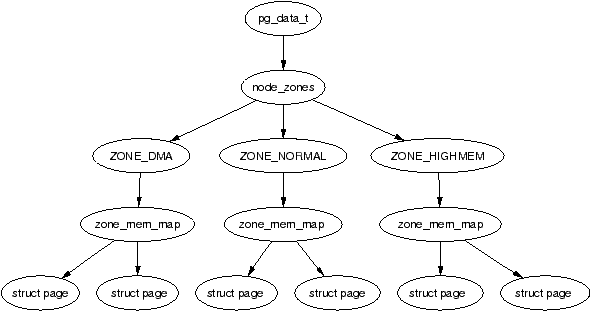
\includegraphics[width=0.8\textwidth]{structrel.png}
  \marginnote{\fig{1}{0 pt}{Relationships between structs. Note that there are multiple
  \texttt{pg_data_t} linked together. (\cite{gorman_2004} pp. 16)}}[-6cm]
\end{center}

To each page frame in the system there is associated a \texttt{struct page}
element that holds all the information needed by the kernel to manage that
frame. All the structs are kept together in a global array called
\texttt{mem_map}.

We are going to describe all the structs represented in Figure 1 starting from
the top of the image.

\marginnote{
    \texttt{pgdat_list} is created incrementally at each
    \texttt{init_bootmem_core} call by prepending each \texttt{pg_data_t}
}[-2cm]


\begin{verbatim}
> include/linux/mmzone.h
typedef struct pglist_data {
    zone_t node_zones[MAX_NR_ZONES];
    zonelist_t node_zonelists[GFP_ZONEMASK+1];
    int nr_zones;
    struct page *node_mem_map;
    unsigned long *valid_addr_bitmap;
    struct bootmem_data *bdata;
    unsigned long node_start_paddr;
    unsigned long node_start_mapnr;
    unsigned long node_size;
    int node_id;
    struct pglist_data *node_next;
} pg_data_t;
\end{verbatim}


\texttt{node_zones[]} holds the \texttt{zone_t} structs for each zone.

\texttt{node_mem_map} is the pointer to the first \texttt{struct page} within
\texttt{mem_map} that belongs to this node (all the other \texttt{struct page}s of the node follow
contiguously in \texttt{mem_map}).

\texttt{node_size} is the total number of page frames belonging to the node.

\texttt{node_next} is the pointer to the next node in the list
\texttt{pgdat_list}.

In the i386 architecture (in which just UMA is supported) the only node
\texttt{contig_page_data} is initialized in \texttt{free_area_init()}
(\texttt{mm/page_alloc.c}) and \texttt{zone_t} fields are filled thanks to the
parameters discovered beforehand through the E820 facility passed to this
function. In the NUMA case (64 bit) node initialization is done in \texttt{setup_arch()} which
indirectly will call \texttt{free_area_init_node()} (\texttt{mm/numa.c}). Both
functions (\texttt{free_area_init*}) will eventually call
\texttt{free_area_init_core()} (\texttt{mm/page_alloc.c}) that performs the
setup of the data structures described below.
\marginnote{\texttt{free_area_init*} is indirectly called by
\texttt{paging_init}}[-36pt]

During the POST phase the BIOS discovers how much physical memory is
available and setups a table called E820, which contains information about how
much physical memory is available and which are the usable regions
(for example in case of shadow-ram initialization the BIOS must inform the
kernel that some portion of memory is not available since it stores BIOS
routines).

\newpage

\begin{verbatim}
> include/linux/mmzone.h
typedef struct zone_struct {
    spinlock_t lock;
    unsigned long free_pages;
    zone_watermarks_t watermarks[MAX_NR_ZONES];
    unsigned long need_balance;
    unsigned long nr_active_pages,nr_inactive_pages;
    unsigned long nr_cache_pages;
    free_area_t free_area[MAX_ORDER];
    wait_queue_head_t *wait_table;
    unsigned long wait_table_size;
    unsigned long wait_table_shift;
    struct pglist_data *zone_pgdat;
    struct page *zone_mem_map;
    unsigned long zone_start_paddr;
    unsigned long zone_start_mapnr;
    char *name;
    unsigned long size;
    unsigned long realsize;
} zone_t;
\end{verbatim}

\texttt{lock} is used to protect the zone from concurrent accesses and is used
by the buddy system to protect the data structures from concurrent access.

\texttt{free_area[]} is an array of structs used for memory allocation by the
Buddy System.

\texttt{zone_mem_map} similarly to \texttt{node_mem_map} points to the first
\texttt{struct page} of \texttt{mem_map} that belongs to this zone.

\begin{verbatim}
> include/linux/mm.h
typedef struct page {
    struct list_head list;
    struct address_space *mapping;
    unsigned long index;
    struct page *next_hash;
    atomic_t count;
    unsigned long flags;
    struct list_head lru;
    struct page **prev_hash;

    #if defined(CONFIG_HIGHMEM) || defined(WANT_PAGE_VIRTUAL)
        void *virtual;
    #endif
} mem_map_t
\end{verbatim}

\texttt{list} is a field used to link this \texttt{struct page} to other
\texttt{struct pages} forming a list of pages satisfying a certain property
(e.g. free pages, dirty pages, locked pages etc.).

\texttt{count} tells the number of processes that are using that page frame. If
it is 0 then it can be put into the list of free pages (usable).

\texttt{flags} describe the status of the frame. 

\texttt{virtual} is used for pages in the highmem area.
virtual then accepts the virtual address of the page if it is mapped to the
kernel address space.

When pages are initialized in \texttt{free_area_init()} the count field is set
to 0 and \texttt{PG_reserved} bit within the \texttt{flags} field is set to 1
so that no memory allocator except for bootmem (which doesn't rely on these data
structures) can allocate that frame. This is done because the Main Memory
subsystem of the kernel will not use the bootmem allocator anymore in its steady
state but new kinds of allocators and therefore it must ensure that there aren't
conflicts between the two.

Frame un-reserving is performed in \texttt{mem_init()}
(\texttt{arch/i386/mm/init.c}) and it will allow the steady state allocator to
start working.

\section{Buddy System}
The kernel subsystem that handles the memory allocation requests for groups of
contiguous page frames is called the \textit{zoned page frame allocator}. \marginnote{(\cite{bovet_cesati_2006} pp. 302),
(\cite{mauerer_2010} pp. 14, Sec. 3.5.1) (\cite{gorman_2004} Chap. 6)  }

The component named "zoned allocator" receives the requests for allocation and
deallocation of dynamic memory. In the case of allocation requests, the
component searches a memory zone that includes a group of contiguous page frames
that can satisfy the request. Inside each zone, page frames are handled by a
component named "buddy system". The buddy system of all zones and nodes are
linked together via the allocation fallback list (\texttt{node_zonelists}).
When a request for memory
cannot be satisfied in the preferred zone or node, first another zone in the
same node, and then another node is picked to fulfill the request.

Free memory blocks in the system are always grouped as two buddies. The buddies can be
allocated independently of each other; if, however, both remain unused at the
same time, the kernel merges them into a larger pair that serves as a buddy on
the next level.

The buddy system uses the \texttt{free_area[]} field of \texttt{zone_t} to perform
memory allocation and deallocation. \texttt{free_area[]} is an array of structs
defined as follows.

\begin{verbatim}
> include/linux/mmzone.h (v. < 2.6.10)
typedef struct free_area_struct {
    struct list_head    free_list;
    unsigned long   *map;
} free_area_t;
\end{verbatim}

\begin{center}
  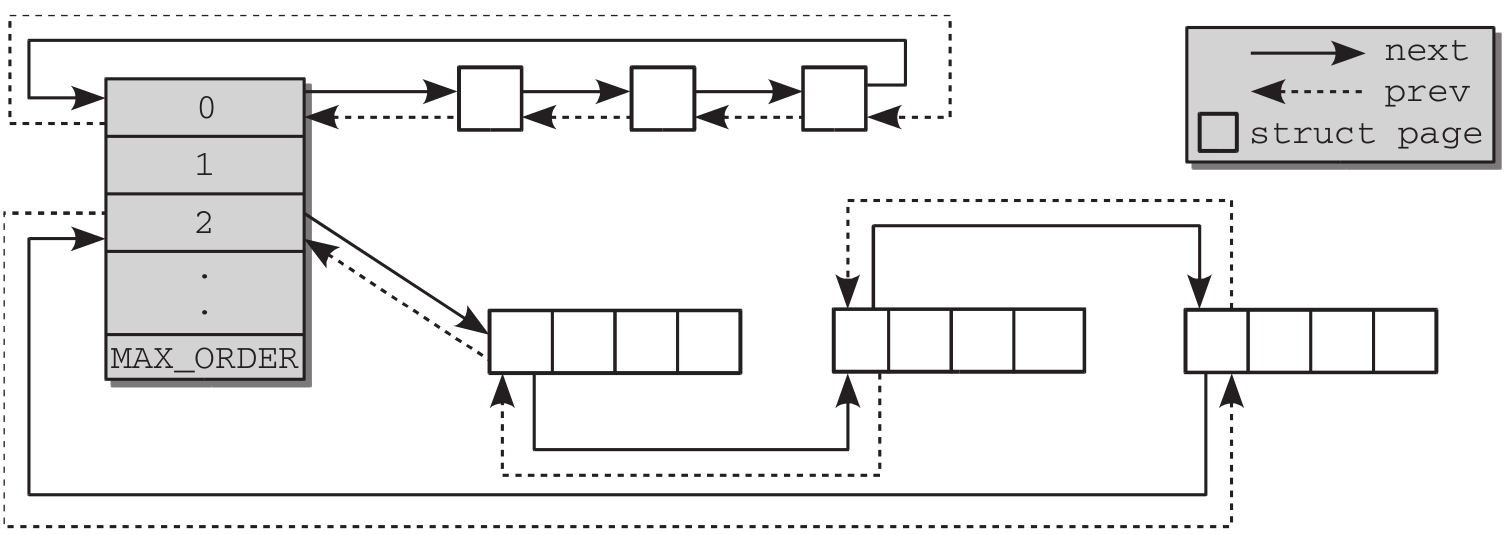
\includegraphics[width=0.8\textwidth]{freearea.png}
  \marginnote{\fig{2}{0 pt}{\texttt{free_area[]} array data structure
  representation within a zone}}[-3cm]
\end{center}

Each entry of the array is associated to an \textit{order} and holds in a list
pointed by \texttt{free_list} memory blocks
of size $2^{order}$ composed of contiguous \textbf{free} \texttt{struct page}s. Therefore
order 0 contains blocks of single pages, order 1 contains blocks of $2^1$ pages,
order 2 blocks of $2^2$ pages, up to \texttt{MAX_ORDER - 1} (\texttt{MAX_ORDER}
usually set to 11). The list is formed by linking the blocks of the same size together through the
\texttt{list} field of the first \texttt{struct page} belonging to the block.

The \texttt{map} field of the struct points to a bitmap used for allocation and
deallocation. Each bit represents a pair of buddies in the current order. It is
set to 0 if both are allocated or both are free and it is set to 1 otherwise.

\marginnote{\textsc{Allocation}}[6pt]
When a request for allocating an area of a given order \texttt{ord} is issued,
the buddy system tries to find a free block inside of
\texttt{free_area[ord].free_list}. If the request can be fulfilled in the
requested order \texttt{ord} then the block is returned and the bit in the
bitmap is toggled. Otherwise the buddy system recursively searches for free
blocks in higher orders, say it is found in \texttt{high_ord > ord},
and splits the block into two blocks (called buddies), one put in the list of
\texttt{high_ord - 1} (also toggling the bits in the bitmap) and the other
recursively split into smaller blocks (buddies) until \texttt{ord} is reached.


\begin{center}
  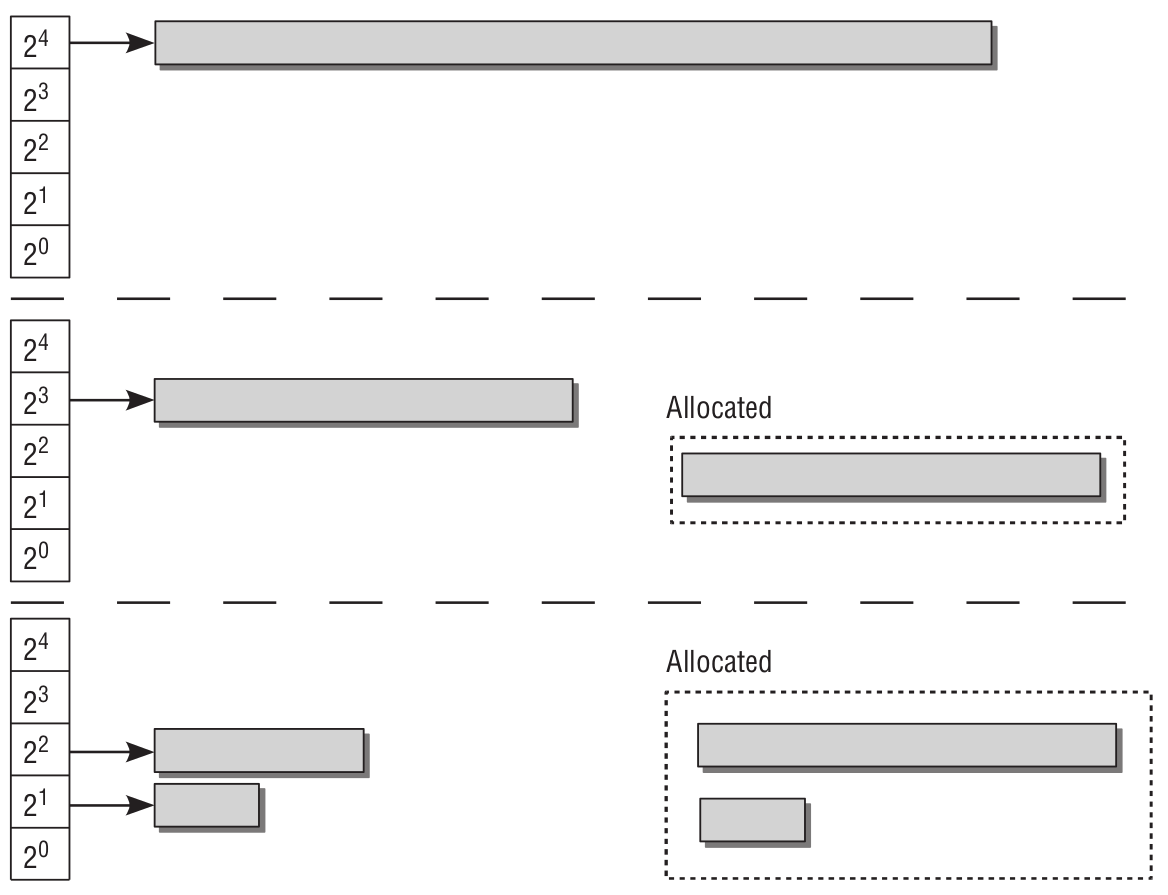
\includegraphics[width=0.8\textwidth]{evol.png}
  \marginnote{\fig{3}{0 pt}{Evolution of \texttt{free_area[]} when first
  requesting a block of order 3 and then of order 1.}}[-6cm]
\end{center}

\marginnote{\textsc{Deallocation}}[6pt]

When the block is later freed, the buddy will be checked. If both are free, the
kernel will try to \textit{coalesce} the buddies together immediately. In the
worst scenario the operation requires \texttt{MAX_ORDER} steps. To detect if the
buddies can be merged or not, the bit corresponding to the affected pair of
buddies in the bitmap is checked. As one buddy has just been freed by this
function it is known that at least one buddy is free. If the bit in the map is 0
after toggling, we know that the other buddy must also be free and thus they can
be merged. Otherwise if the bit is 1, the other buddy is in use therefore the
buddies cannot be merged and the block goes into its order list.

All the memory operations performed by the buddy system require the acquirement
of the \texttt{lock} found in \texttt{zone_t} therefore it can be a bottleneck
for the responsiveness of the system since there can be contentions on the
spinlock.

Even though the algorithm is very fast, the frequent allocation and release of
page frames and blocks may lead to a situation in which several page frames are
free in the system but they are scattered (not contiguous) throughout the
physical address space.
Single reserved pages that sit in the middle of an otherwise large continuous free range can
eliminate coalescing of this range very effectively.

The finalization of memory management initialization is done in
\texttt{mem_init()}.

\begin{verbatim}
> arch/i386/mm/init.c
mem_init()
    ...
    free_pages_init()
        ...
        > mm/bootmem.c
        free_all_bootmem()
            free_all_bootmem_core() {
                ...
                for (i = 0; i < idx; i++, page++) {
                    if (!test_bit(i, bdata->node_bootmem_map)) {
                        count++;
                        ClearPageReserved(page);
                        set_page_count(page, 1);
                        __free_page(page); //decrements page count and if 0
                                           //adds page into the free list
                    }
                }
                ... // free also bootmem map
            }
\end{verbatim}

For each unallocated page in bootmem, the page flag \texttt{PG_reserved} is
cleared (it was previously set on initialization by
\texttt{free_area_init()} as said previously) and the \texttt{count} is set to 1
in order to fake \texttt{__free_page()} into thinking that this is an ordinary
deallocation for the buddy system which on decrementing \texttt{count} and
\marginnote{(\cite{gorman_2004} Chap. 6), (\cite{mauerer_2010} Sec 3.5.4)}[2cm]
checking that is 0 will put it into the free list.

\subsection{Zoned Allocator APIs}


\begin{verbatim}
> mm/page_alloc.c
// Allocation
alloc_pages(gfp_mask, order)
    Used to request 2^order contiguous page frames. It returns struct
    page * of the first page of the block

get_zeroed_page(gfp_mask)
    it expands to alloc_pages(gfp_mas | __GFP_ZERO, 0) but instead of
    returning a struct page * it returns the linear address of the page
    frame allocated. The contents of the page are set to 0

__get_free_page(gfp_mask)
    Allocates one page frame and returns its linear addres

__get_free_pages(gfp_mask, order)
    similar to alloc_pages(gfp_mask, order) but returns the linear
    address of the first page frame of the block

// Deallocation
free_page(addr)
    frees a page given its linear address

free_pages(addr, order)
    frees a block given its linear address and its order

__free_pages(page, order)
    given a struct page * if its PG_reserved is set to 0 (page not
    reserved) decreases the count field and if it becomes 0 it assumes
    that 2^order contiguous page frames starting from the one corresponding
    to page are no longer used

__free_page(page)
    expands to __free_pages(page, 0)
\end{verbatim}

\begin{center}
  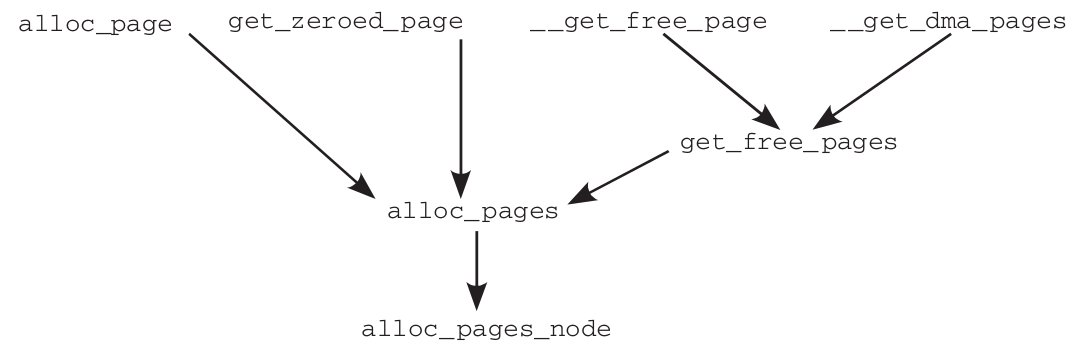
\includegraphics[width=0.8\textwidth]{allrel.png}
  \marginnote{\fig{4}{0 pt}{Relationships between allocating functions}}[-3cm]
\end{center}


[prolinkern pp. 220 for flags]

The \texttt{gfp_mask} parameter is a mask consisting of a set of flags that
specifies to the zoned allocator the allocation context, such as \textit{zone
modifiers} of the allocation (\texttt{__GFP_DMA, __GFP_HIGHMEM}) or others such
as 

\begin{verbatim}
GFP_ATOMIC
the allocation cannot be interrupted (the process cannot be put into sleep)
since this is a urgent allocation.

GFP_KERNEL and GFP_USER
respectively used to allocate kernel memory and userspace memory

GFP_NOFS (previously GFP_BUFFER)
generic page, usually used to allocate a buffer

\end{verbatim}


\section{High Memory}

High memory allocations can be performed only through the subset of APIs
described above which return \texttt{struct page *}. This is done because page
frames in the \texttt{ZONE_HIGH} area (above 896MB) do not have a permanent
mapping in the linear address space of the kernel.

The kernel uses three different mechanisms to map page frames in high memory;
they are called \textit{permanent kernel mapping, temporary kernel mapping} and
\textit{noncontiguous memory allocation} (this one described later). Memory
allocation for high memory  is performed through \texttt{alloc_pages()} and \texttt{alloc_page()} APIs described above. These APIs return the
linear address of the page descriptor (\texttt{struct page *}) of the first
allocated page frame which always exist because all page descriptors are
allocated in \textit{low memory} (\texttt{0:896MB}). The kernel then uses part
of the last 128MB of its linear address space to map high-memory page frames.
Trivially this kind of mapping is temporary otherwise only 128MB of high memory
would be accessible.

\begin{description}
    \item \texttt{vmap(struct page **pages, int count, unsigned long flags,
        pgprot_t prot)} \marginnote{(\cite{mauerer_2010} pp. 250)}

        Given an array of \texttt{struct page *} (even not contiguous) creates
        the entries in the page tables to access the pages through a
        virtually contiguous space. When freeing \texttt{vmap}ped area through
        \texttt{vunmap} eventually \texttt{vmfree_area_pages}
        (\texttt{mm/vmalloc.c}) will be called which will also flush the TLB on
        all cores.

    \item \texttt{kmap(struct page *)} \marginnote{(\cite{mauerer_2010} Sec.
        3.5.8)}

        Given a page descriptor, maps the physical addresses of that page to
        the virtual address space of the kernel in highmem starting with virtual
        address \texttt{PKMAP_BASE}. These pages are also
        known as "Permanent Kernel Mappings". There is a dedicated Page Table
        (last level) in the kernel page tables of which address is stored in
        \texttt{pkmap_page_table} to handle this kinds of mappings.

        An array of
        counters \texttt{pkmap_count[LAST_PKMAP]} each referring to an entry of
         \\ \texttt{pkmap_page_table} is used for management. If a counter is 0 it
        means that the corresponding PTE is not used for mapping any high-memory
        page frame and is usable. If it is 1 it means that the PTE does not map any
        high-memory page frame but it cannot be used since the corresponding TLB
        entry has not been flushed since its last usage. If the counter is $n$
        the corresponding PTE maps a high-memory page frame which is used by
        exactly $n-1$ kernel components ($n-1$ components have called
        \texttt{kmap} on the same \texttt{struct page *}. Note that if a page
        frame was already \texttt{kmap}ped and \texttt{kmap} is called again on
        the very same page frame, then the second call will return the same
        virtual address of the first).

        When mapping a page frame with no corresponding virtual address the
        function tries to find an empty PTE in \texttt{pkmap_page_table} (i.e. a
        PTE with counter 0), creates the entry, sets its counter to 2, 
        and returns the virtual address assigned. When unmapping through
        \texttt{kunmap} the counter is decremented (therefore it will be 1 when
        no kernel thread references that page anymore). The TLB is flushed on all
        cores through \texttt{flush_tlb_all()} only when all the PTEs have
        counter 1. No errors caused by TLB caching can arise since if over time
        two threads perform \texttt{kmap$_1$ -> kunmap$_1$ -> kmap$_2$} (where
        the subscript tells the id of the thread performing the call and arrows
        indicate the temporal sequence of events) with in betweeen them any
        kind of operations, and both \texttt{kmap$_1$} and \texttt{kmap$_2$}
        return the same virtual address there must have been a
        \texttt{flush_tlb_all()} in between the first unmapping and the second
        mapping according to the algorithm.

        Note that in case of not available PTEs the kernel thread issuing a
        \texttt{kmap} might be put to sleep until one is available
        (\texttt{kunmap} issued). Also
        since the number of available PTEs are those fitting in one page frame
        the function must be used for mappings of not too prolonged time.

\newpage

    \item \texttt{kmap_atomic(struct page *page, enum km_type type)}

        The \texttt{kmap} function described above must not be used in interrupt
        handlers because it can lead to sleep. The kernel therefore provides this
        alternative mapping function that executes atomically. When a thread
        calls this function it becomes not preemptable until it issues
        \texttt{kunmap_atomic}. To make a thread not preemptable the function
        increases its \texttt{preempt_count} field. Before returning the
        function ensures that the TLB of the processor on which the thread runs
        doesn't have cached anything on the virtual address it is going to
        return by calling \texttt{__flush_tlb_single(vaddr)}. By this fact, the
        mapping is not visible to other processors. The function uses a portion
        of virtual memory called fixmap.

\end{description}


\section{NUMA Allocation Policies}
\label{sec:NUMA Allocation Policies}

Starting from kernel v. 2.6.18, there were added system calls that allowed userspace
to specify a policy to honor during allocations. Note that such policies are
followed also by the functions described above. The implementation of this
system calls can be found in \texttt{mm/mempolicy.c} through the macro
\texttt{SYSCALL_DEFINE*} which will be explained in future lectures.
By policy it is meant on which
node the kernel should allocate memory in a NUMA system.
One of the main functions is
\texttt{set_mempolicy(int mode, unsigned long *nodemask, unsigned long maxnode)}
which sets the memory policy of the calling thread. The \texttt{mode} parameter
can be one between

\begin{description}
    \item \texttt{MPOL_DEFAULT}

        Sets the policy for the calling thread to the system's default policy
        which tries to allocate memory from the node requesting it and then to
        close nodes. When specified in the \texttt{mbind} function (see below)
        it follows the thread policy.

    \item \texttt{MPOL_BIND}

        This mode specifies that memory must come from the
        set of nodes specified by the policy through \texttt{nodemask} and 
        \texttt{maxnode}.  Memory will be allocated from
        the node in the set with sufficient free memory that is closest to
        the node where the allocation takes place.

    \item \texttt{MPOL_INTERLEAVED}

        This mode specifies that page allocations be
        interleaved, on a page granularity, across the nodes specified in
        the policy.

    \item \texttt{MPOL_PREFERRED}

        This mode specifies that the allocation should be
        attempted from the single node specified in the policy.  If that
        allocation fails, the kernel will search other nodes, in order of
        increasing distance from the preferred node based on information
        provided by the platform firmware.
\end{description}

\texttt{mbind(void* addr, unsigned long len, int mode, unsigned long *nodemask,
\\ unsigned long maxnode, unsigned flags)} sets a NUMA policy for a range of
addresses starting from \texttt{addr} to \texttt{addr + len}.

The system call \texttt{move_pages(pid_t pid, unsigned long nr_pages, void **pages,
\\ const int *nodes, int *status, int flags)} is defined in
\texttt{mm/migrate.c} to allow to move pages from one NUMA node to another. Note
that this is an expensive operation that requires the cache controllers of the
various cores to perform the migration of pages working at 64Bytes per time. For
more information about NUMA policies refer to \\
\texttt{Documentation/vm/numa_memory_policy.txt} and manpages.

\section{Conclusions}
\label{sec:Conclusions}

In this lecture various parts of the memory management of the linux kernel were
explored. While the code seen in the previous lectures were about specific,
older versions of the kernel, the concept shown in this lecture apply also to
modern versions of it. One main observation has to be done: as anticipated the
concept of high memory thankfully is not present in 64 bit systems since the virtual
address space of the kernel is more than enough to address all the possible
physical memory.

The concept of NUMA system is introduced in the kernel which brings in new
problems and
interfaces in the system programming world such as the concept of NUMA policies.
In linux UMA systems are treated as NUMA systems having just one node. In this
context allocations are driven by NUMA policies combined with the Buddy Sytems.

When an allocation needs to be performed, the current NUMA policy for the thread
issuing the request is queried combined with the eventual zone modifier defined
by the \texttt{gfp_mask} of the request to choose the Buddy System that has to
fulfill the request. There is one Buddy System per zone within a node and the
requests to one buddy are serialized, i.e. managed through the lock in
\texttt{zone_t}.



\newpage
\bibliography{Lec6}
\bibliographystyle{plainnat}
\end{document}
